\documentclass[11pt,twocolumn]{article}
\usepackage[breaklinks]{hyperref}
\usepackage{latexsym}
\usepackage[letterpaper]{geometry}
\geometry{verbose,tmargin=1in,bmargin=1in,lmargin=1in,rmargin=1in}
\setlength{\columnsep}{0.5in}

\usepackage{graphicx}

\renewcommand{\familydefault}{\sfdefault}
\usepackage{helvet}
\usepackage{sansmath}
\usepackage{inconsolata}
\usepackage{microtype}

\renewcommand{\theenumi}{\alph{enumi}}
\renewcommand{\labelenumi}{\theenumi.}

\begin{document}
\title{\textbf{GenomeAssist}\\
       An Online Sequence Aligner Comparison Tool}
\author{Mansi Arora and Roger Que}
\date{2013--12--16}
\maketitle


\begin{abstract}
We present GenomeAssist, a Web-based tool for the comparison of
sequence aligners.
GenomeAssist provides genomicists with a graphical interface to run
existing alignment tools on a backend cluster, without needing any
command line knowledge or provisioning of local shell accounts.
Results are aggregated into user-friendly visualizations that allow
at-a-glance views of accuracy and runtime performance.
\end{abstract}


\section{Background}
Sequence alignment is, perhaps more than any other class of algorithms,
fundamental to genomic data processing.
A wide variety of approaches to the problem have emerged, variously
motivated by the increasingly parallel nature of scientific computing,
the discovery of new algorithms and data structures such as the
FM-index, and changes in how sequencers themselves extract and present
sequence data.
In particular, the shift towards next-generation sequencers, which trade
an overall higher throughput and lower cost for shorter individual
reads, has given rise to many different alignment algorithms and tools
geared towards their output \cite{Li:2010}.
With the large number of available alignment tools, questions arise
about which one of them is most suitable for any particular data set.

Unfortunately, alignment tools have a relatively high barrier to entry.
The first problem is one of resources:
The amounts of data and computational power required to evaluate
a set of sequence aligners against any given scenario are often too
cost-prohibitive for a single user.
This problem may be ameliorated in institutional environments with the
availability of a computing cluster specifically geared towards research
use, shared by a group or a department.
However, this does nothing to address the second problem, which is one
of general user accessibility.
As many aligners are designed to be run on ``headless'' servers with no
direct display output, they are generally instead invoked by logging in
remotely to a command-line interface, and then specifying the preferred
parameters by text strings.
This process carries a high cognitive overhead for users unaccustomed to
such software, overhead that is unrelated to the immediate problem of
sequence alignment.
In addition, there may be network security questions involved in the
provisioning of accounts; for example, administrators may be reluctant
to provide full shell access to a cluster when users should only be able
to run alignment tools.

For this reason, some sequence alignment and search tools are available
through Web-based interfaces, which can be launched through a browser.
The most well-known of these tools is almost certainly BLAST, which is
available through the Web site of the National Center for Biotechnology
Information \cite{BLAST}.
Other frontends have been developed for other aligners.
Of particular note is Crossbow \cite{Crossbow}, which is designed for
whole-genome resequencing analysis.
The Crossbow pipeline combines the Bowtie aligner with the SoapSNP
genotyper, and allows for the immediate spawning of jobs on Amazon EC2.
Additional tools exist for aligners such as LALIGN/PLALIGN, the CLUSTAL
toolkit, and MAFFT.

One major limitation of many of these Web frontends is that they do not
make any attempt to make the aligners more accessible to a wider
audience, but simply make them available for non-local usage.
For example, Crossbow simply provides a text entry field for ``Bowtie
options'' that are passed directly on the Bowtie command line, requiring
the user to read the manual and arrive at the appropriate argument
string on his or her own.
Output, too, is frequently presented as raw text, instead of in a format
that can be immediately understood at a glance.

A more fundamental problem, however, lies in the fact that no existing
Web-based tool allows the user to directly compare different alignment
algorithms, meaning that a genomicist who wishes to investigate the
performance of various aligners receives no help in efficient decision
making.
As different aligners have significantly different performance profiles,
whether specified in terms of accuracy and error reporting, or in terms
of computing resources such as memory and CPU time, it is important for
genomicists to understand these differences.
However, configuring, installing, and running a large collection of
tools can be a tedious task, made more troublesome by the accessibility
issues mentioned previously.

In order to fill this unmet need, we have created GenomeAssist, an
online tool specifically geared towards the comparison of sequence
aligners.
GenomeAssist provides a common, consistent frontend to various alignment
tools, allowing genomicists to easily simultaneously run several aligner
instances against a single common set of read and reference data.
Results are presented through a graphical frontend that normalizes the
differing output formats into charts and graphs that allow for quick
visual comparisons, while still allowing the user to delve further into
each aligner's particular output should the need arise.
New tasks can be easily created based on the parameters used for
previous runs, allowing users to iteratively arrive at the optimal
settings for their specific scenario.


\section{Feature overview}

The GenomeAssist interface is centered on the creation of \textit{jobs},
which are collections of aligner runs operating on a shared read file
and reference genome.
Each run contained within a job is referred to as an \textit{aligner
task}, or simply a \textit{task}.
GenomeAssist requires that all tasks be part of a job, although a job
may contain only a single task.
As detailed in Section~\ref{sec:detail}, a job's results can be viewed
in aggregate, or broken down by each component task.
Currently, GenomeAssist implements a minimal user account system, which
restricts the viewing of job results to the creating user.


\subsection{Creating jobs}

\begin{figure*}
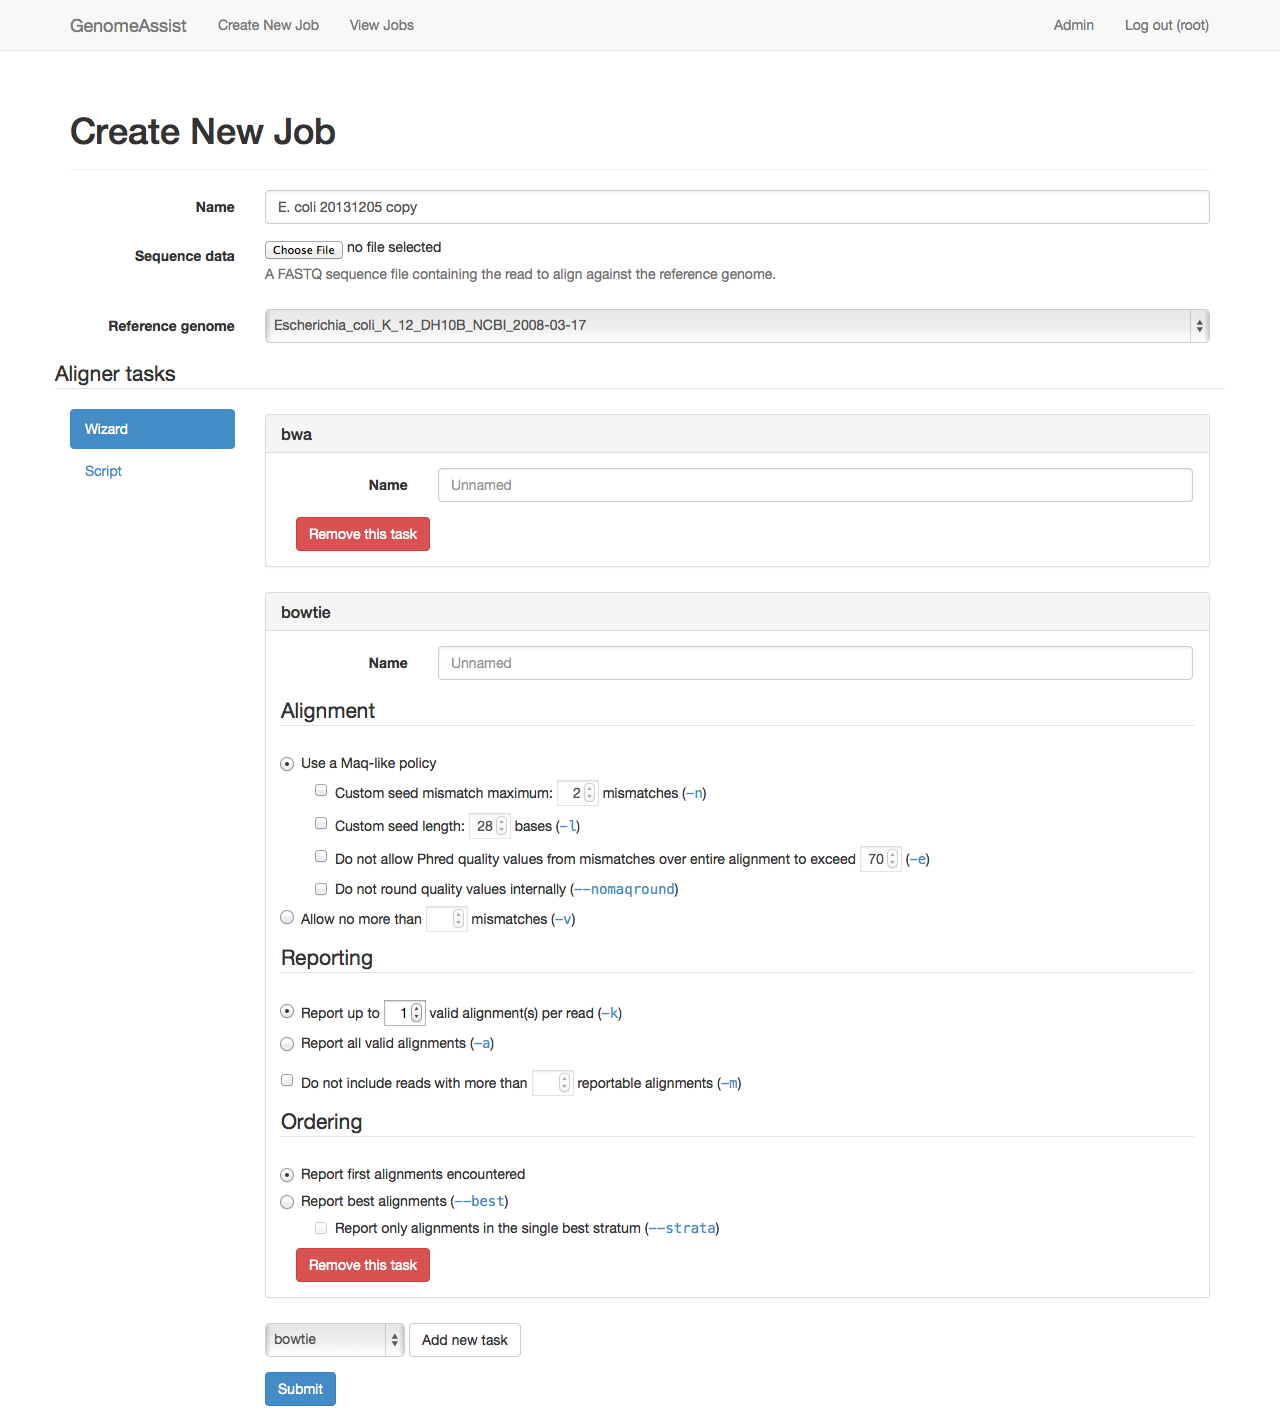
\includegraphics[width=\textwidth]{screenshots/create-prefill-full}

\caption{
    \label{fig:create}
    GenomeAssist's job creation interface, showing options available
    for Bowtie.
}
\end{figure*}

An overview of GenomeAssist's job creation interface is shown in
Figure~\ref{fig:create}.
At the top of the provided form are basic fields for setting an
optional job name that will be used in the rest of GenomeAssist,
uploading a read file, and specifying a reference genome.
This read file and reference genome will be used for all of the tasks
belonging to this job.

The majority of the page is dedicated to the aligner task creation form.
By default, a wizard-like interface is provided, through which the user
can graphically add new tasks and specify their respective options.
For users already familiar with the command-line operation of a specific
aligner, CLI option names such as \texttt{-k} or \texttt{--best} are
also indicated, with links to the aligner's manual page if available.
Multiple tasks using the same aligner may be specified, allowing users
to run a single aligner with different options.
This may be useful, for example, if the user wishes to compare different
seed sizes for a hash table--based aligner, and select a value with an
acceptable tradeoff between accuracy and speed.

More advanced users may directly edit a job's \textit{task script} by
selecting the script view.
The script defines the list of tasks and their respective options in a
serialized JSON format, and is what is actually processed by the job
scheduling backend.
For example:
\begin{verbatim}
    [{
        "aligner": "bwa",
        "name": "BWA task 1",
        "options": "[omitted]"
    }, {
        "aligner": "bowtie",
        "name": "Bowtie task 2",
        "options": "[omitted]"
    }]
\end{verbatim}
This feature allows for a more compact specification of the parameters
passed to a job, useful in cases where job information is being sent by
some external textual medium such as e-mail.
(Note that users do not need to use task scripts to create a new job
based on the specifications of a job that they have already created;
instead, they may create copies of existing jobs from the job output
page, as outlined in Section~\ref{sec:detail}.)
The user is not required to use the wizard to individually specify each
option, but can instead simply paste the job script into the appropriate
text entry field.
Once entered, the graphical wizard's fields are resynchronized with the
options given in the script, so that the user may switch back to the
wizard view and make further changes to task options without needing to
modify the serialized script.


\subsection{Viewing job output}
\label{sec:detail}

\begin{figure*}
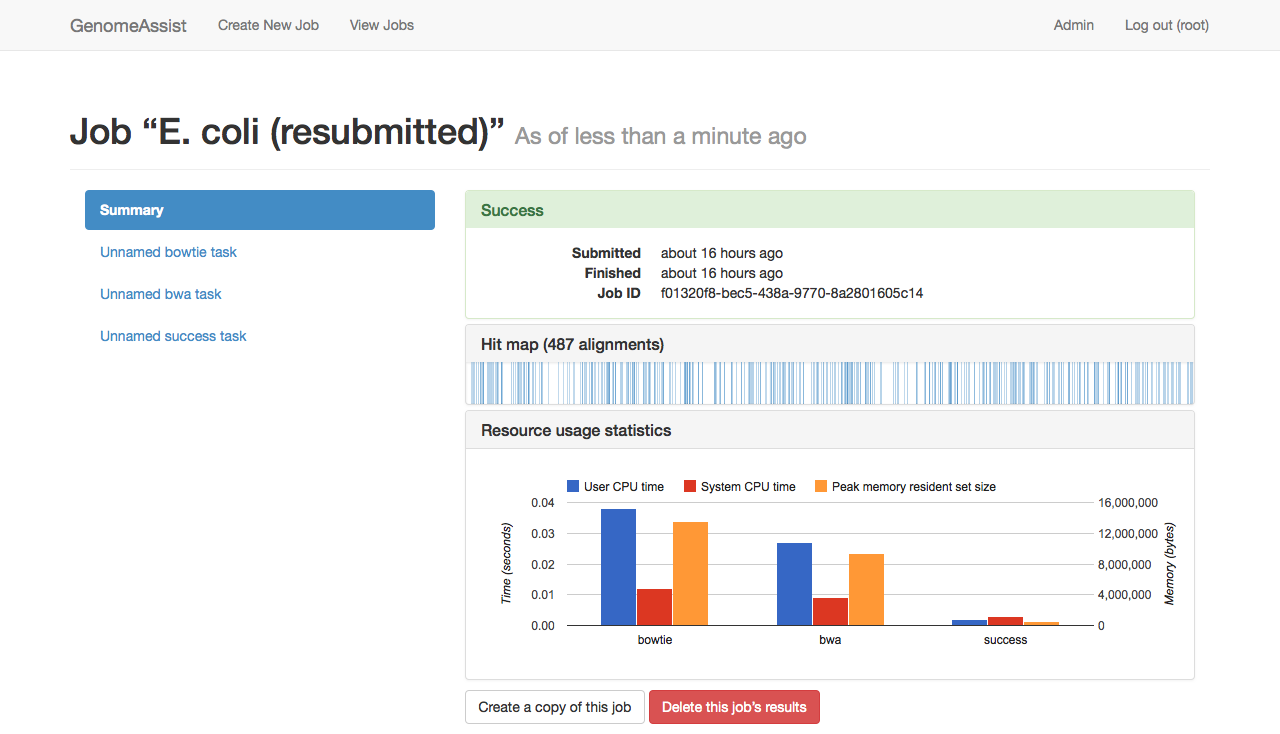
\includegraphics[width=\textwidth]{screenshots/detail-full}

\caption{
    \label{fig:detail}
    GenomeAssist's job detail page, showing a sample alignment of
    1,000 reads against the \textit{Escherischia coli} genome.
}
\end{figure*}

After submitting a job to GenomeAssist, the user can view its current
status and any eventual output on the job detail page.
Upon a job's successful completion, a summary visualization is shown, as
in Figure~\ref{fig:detail}, composed of a \textit{hit map} and resource
usage statistics.

The hit map gives a linear view of all loci to which a read successfully
aligned in at least one of the aligner tasks.
Alignments are indicated by vertical lines, colored by their average
quality value over all tasks.
Darker lines indicate higher quality values.
Individual alignments may be hovered over with the mouse to display
their exact position and quality value information.

Below the hit map is a chart displaying the comparative resource usage
of each aligner task.
Currently, the amount of userland and system CPU time consumed, as well
as peak memory utilization, are displayed on the chart.
This allows the user to quickly gauge the relative efficiency of each
aligner task, in comparison to its alignment accuracy.

At the bottom of the summary view are buttons allowing the user to
create a copy of this job, which pre-fills the job creation form with
the reference genome and aligner options that were used in the job
currently being viewed, or delete the job's results, hiding them from
the default job listing.
Job result deletion may be undone at any time, assuming that the deleted
job's information has not been pruned from the database.

Status information, hit maps, and resource usage statistics are also
available for individual tasks within a job, assuming that they have
completed successfully.
In addition, the raw textual output of each aligner is displayed,
allowing further analysis to be performed with external tools.


\section{Implementation}
\label{sec:implementation}

GenomeAssist is implemented as a Python application, using the Django
Web application framework \cite{Django} and the Celery distributed task
library \cite{Celery}.
In our testing, we used an on-disk SQLite database to store job and task
information, along with a RabbitMQ message broker for coordinating task
execution, although any combination supported by the above libraries
should be sufficient.
Currently, the resource usage tracking functionality requires that
GenomeAssist be run on a Unix-like platform; it has been tested to work
on Mac OS X and Ubuntu Linux.

Jobs are handled using a MapReduce-like paradigm, with individual
aligner tasks being spun off to individual worker processes, and their
results collated by a final aggregation task before being presented to
the user.
Aligner tasks are implemented as Celery task classes with two bespoke
methods.
The first, \texttt{parse\_options}, is used to transform the URL-encoded
options string passed in by the GenomeAssist frontend, along with the
read and reference genome paths, into a list of command-line arguments.
These arguments are then used to spawn a subprocess on the same machine
as the Celery worker process.
If the aligner does not encounter any errors, its output is passed to
the the second custom method, \texttt{parse\_output}, which transforms
it into a format usable by the GenomeAssist frontend.
A standard function for converting SAM output to this format is
provided with GenomeAssist.
Finally, when all aligner tasks have completed, the collected results
are passed to the aggregator, which outputs data suitable for use by the
visualizations on a job's summary page.

In its current incarnation, GenomeAssist shares data among the frontend
and worker processes, such as reference genome indexes and uploaded read
files, by means of mounted network shares on each host.

The frontend user interface is largely built on Twitter Bootstrap and
jQuery, with some charting functionality provided by Google Charts.
The use of these standard UI frameworks minimizes browser compatibility
issues, allowing GenomeAssist to be used more easily in heterogeneous
computing environments.

The GenomeAssist source code, including basic setup instructions, is
available at \url{https://github.com/query/genomeassist}.


\section{Future work}

Currently, GenomeAssist supports BWA~\cite{BWA} and version 1.0 of the
Bowtie aligner \cite{Bowtie}, with the graphical wizard interface only
available for Bowtie.
Some features of these aligners are also not yet available; for
instance, GenomeAssist does not support the alignment of paired-end
reads.
GenomeAssist can easily be extended to support additional command-line
aligners, however, by providing an HTML wizard form and implementing a
Celery task class with appropriate methods for parsing options and text
output, as outlined in Section~\ref{sec:implementation}.

GenomeAssist implements data sharing by means of locally mounted network
file shares.
Although Unix filesystem drivers are generally available for distributed
file systems such as HDFS and Amazon S3, more direct support of these
storage backends would be useful in situations where GenomeAssist is
being installed by users in restricted computing environments who cannot
or do not wish to install and configure these drivers.


\begin{thebibliography}{1}

\bibitem{BLAST}
{BLAST}: Basic local alignment search tool.
\newblock National Center for Biotechnology Information.
  \url{http://blast.ncbi.nlm.nih.gov/}.

\bibitem{Django}
Django: The {Web} framework for perfectionists with deadlines.
\newblock Django Software Foundation. \url{https://www.djangoproject.com/}.

\bibitem{Crossbow}
Ben Langmead, Michael Schatz, Jimmy Lin, Mihai Pop, and Steven Salzberg.
\newblock Searching for {SNPs} with cloud computing.
\newblock {\em Genome Biology}, 10(11):R134, 2009.

\bibitem{Bowtie}
Ben Langmead, Cole Trapnell, Mihai Pop, and Steven Salzberg.
\newblock Ultrafast and memory-efficient alignment of short {DNA} sequences to
  the human genome.
\newblock {\em Genome Biology}, 10(3):R25, 2009.

\bibitem{BWA}
Heng Li and Richard Durbin.
\newblock Fast and accurate short read alignment with {Burrows--Wheeler}
  transform.
\newblock {\em Bioinformatics}, 25(14):1754--1760, Jul 2009.

\bibitem{Li:2010}
Heng Li and Nils Homer.
\newblock A survey of sequence alignment algorithms for next-generation
  sequencing.
\newblock {\em Briefings in Bioinformatics}, 11(5):473--483, 2010.

\bibitem{Celery}
Ask Solem and contributors.
\newblock Celery: Distributed task queue.
\newblock \url{http://www.celeryproject.org/}.

\end{thebibliography}


\end{document}
